\documentclass[twocolumn]{article}
\usepackage[margin=0.75in]{geometry}

% Mock IEEE commands for compilation with article class
\newcommand{\IEEEauthorblockN}[1]{\large\textbf{#1}\\}
\newcommand{\IEEEauthorblockA}[1]{\small\textit{#1}\\}
\newenvironment{IEEEkeywords}{\vspace{1em}\noindent\textbf{\textit{Keywords---}}}{\vspace{1em}}

\usepackage{amsmath}
\usepackage{graphicx}
%\usepackage{siunitx}
\newcommand{\SI}[2]{#1\,#2}
\newcommand{\degree}{\ensuremath{^\circ}}
\usepackage{hyperref}
\usepackage{cite}
\usepackage{booktabs}
\usepackage{float}

\begin{document}

\title{Satellite-Guided Machine Learning Bias Correction of CMIP6 Significant Wave Height Projections over the Indian Ocean}

\author{%
  Pritam Anand\textsuperscript{1}\\%
  \textsuperscript{1}DA-IICT, Gandhinagar, India\\%
  Email: pritam\_anand@dau.ac.in%
}

\maketitle

\begin{abstract}
Accurate projections of ocean wave climate are critical for assessing coastal risks and designing resilient maritime infrastructure under climate change. However, significant wave height (SWH) fields derived from CMIP6-based model chains exhibit systematic biases when compared with satellite altimeter observations, particularly in coastal regions and enclosed basins. This study develops and evaluates a satellite-guided machine learning post-processing framework to correct biases in CMIP6 SWH projections over the Indian Ocean (50°--110°E, 70°S--70°N). Using a Random Forest regressor (100 estimators) trained on the overlap period 2015--2020 between a CMIP6 proxy SWH product and multi-mission satellite altimeter SWH (SARAL/AltiKa, Sentinel-3, Jason-3), we learn a non-linear mapping from model SWH, latitude, longitude and month to observed SWH on a common grid. The trained model is then applied to an independent evaluation period to mimic bias correction for future projections. For the pilot period (2015--2020), the correction reduces the regional mean RMSE from \SI{0.599}{m} to \SI{0.308}{m} (48\% reduction) and achieves an $R^2$ of 0.933 against satellite observations, with the mean bias reduced from \SI{+0.162}{m} to negligible levels. These results demonstrate that machine learning post-processing can substantially improve the fidelity of CMIP6-based wave climate projections using existing satellite products, and provides a transferable workflow for bias-corrected SWH scenarios under future CMIP6 emission pathways.
\end{abstract}

\begin{IEEEkeywords}
Significant wave height, CMIP6, bias correction, satellite altimetry, Random Forest, machine learning, Indian Ocean
\end{IEEEkeywords}

\section{Introduction}

Ocean surface waves modulate air--sea fluxes of momentum, heat and mass and play a central role in coastal flooding, erosion and offshore engineering design \cite{lemos2020}. Reliable projections of future significant wave height (SWH) are therefore essential for climate-resilient coastal planning. In practice, wave climate projections are often constructed by forcing spectral wave models with surface winds from global climate models participating in CMIP6, or by using CMIP6-derived wave products directly. Despite the increased realism of CMIP6, large-scale and regionally structured SWH biases remain when these products are compared against reanalyses and satellite altimetry, especially near coasts and in semi-enclosed seas.

Bias correction is now recognized as a necessary step for wave climate applications. Classical approaches such as the delta method, empirical quantile mapping (EQM) and empirical Gumbel quantile mapping (EGQM) have been shown to substantially reduce errors and improve the representation of extremes \cite{lemos2020}. However, these techniques are typically univariate, often assume stationary bias structures between historical and future periods, and do not explicitly exploit spatial or seasonal covariates.

In parallel, there has been rapid progress in machine learning (ML) post-processing of numerical weather prediction and wave forecasts. Recent studies have demonstrated that tree-based ensembles and deep learning architectures can successfully correct systematic model errors, often achieving double-digit reductions in RMSE and bias for SWH forecasts \cite{sun2022}. In particular, deep convolutional architectures such as U-Net variants have been used to correct gridded SWH from WAVEWATCH III over the Northwest Pacific, yielding large improvements in performance during typhoon conditions \cite{sun2022}.

This paper focuses on a simpler but practically important setting: bias correction of monthly CMIP6-based SWH over the Indian Ocean using satellite altimeter observations as reference. Instead of correcting short-range forecasts, we design an ML post-processing model that maps historical CMIP6 SWH, geographical coordinates and month-of-year to observed SWH on a common grid, and then apply this mapping to unseen years as a proxy for future scenarios.

The specific objectives are:
\begin{itemize}
  \item to quantify the magnitude and spatial structure of CMIP6 SWH biases relative to satellite altimeter observations over the Indian Ocean;
  \item to develop a Random Forest based bias correction model that uses model SWH, latitude, longitude and month as predictors of observed SWH;
  \item to evaluate the correction on an independent test period and quantify improvements in RMSE, bias and correlation;
  \item to outline how the trained model can be applied to generate bias-corrected SWH projections for future CMIP6 emission pathways.
\end{itemize}

\section{Data and Study Region}
 
 \subsection{Model data}
 
 We use a CMIP6-derived significant wave height product (\texttt{cowcliphs.nc}) as a proxy for climate model projections. The ensemble includes 15+ ESMs (e.g., ACCESS-ESM1-5, CESM2, CNRM-ESM2-1, EC-Earth3, GFDL-ESM4, IPSL-CM6A-LR, MIROC6, MPI-ESM1-2-HR, NorESM2-LM, UKESM1-0-LL) with complete SSP scenario coverage (SSP1-2.6, SSP2-4.5, SSP3-7.0, SSP5-8.5). The dataset provides monthly SWH over the Indian Ocean (50°--110°E, 70°S--70°N) on a regular latitude--longitude grid with nominal horizontal resolution of approximately \SI{0.5}{\degree}. The initial dataset contains 151,200 grid points, which after land masking and quality control reduces to 85,796 valid ocean data points. In the workflow, the original coordinate and variable names are renamed to a common convention with dimensions \texttt{time}, \texttt{lat}, \texttt{lon} and variable \texttt{swh}.
 
 \subsection{Satellite altimeter observations}
 
 As observational reference we employ a gridded daily mean SWH product (\texttt{io-altimeter.nc}) from multi-mission satellite altimetry over the Indian Ocean. The dataset integrates missions including SARAL/AltiKa, Sentinel-3A/B, Sentinel-6A, Jason-3, Cryosat-2, and Haiyang-2B, ensuring high spatial sampling and robust quality control (100\% ocean coverage, error estimates 3.6--148.4 mm). These data are provided on a \SI{2.0}{\degree} grid, which serves as the common analysis grid for this study. After renaming to the same coordinate convention, the satellite dataset defines the target SWH field for both diagnostic evaluation and training of the correction model.
 
 \subsection{Temporal coverage and overlap}
 
 Both datasets are available over the period January 2015 to December 2020 for the pilot study, with extended records available up to 2024. To ensure strict temporal alignment, we resample each dataset to monthly means using a month-start sampling interval and then intersect the resulting time coordinates. This yields a consistent multi-year monthly time series of collocated model and observed SWH fields over the Indian Ocean. The temporal split strategy allocates 2015--2018 (67\% of data, 57,228 samples) for model training and 2019--2020 (33\% of data, 28,568 samples) for independent validation, simulating the application to future unseen scenarios.
 
 \section{Methods}
 
 \subsection{Pre-processing and regridding}
 
The analysis and correction workflow is implemented in Python using \texttt{xarray}, \texttt{numpy}, \texttt{pandas} and \texttt{scikit-learn}. After renaming coordinates, we first restrict both model and observational datasets to the common time window 2015--2020 and form monthly means. The model SWH fields are then interpolated to the observational grid via bilinear interpolation using the \texttt{interp\_like} function, producing a regridded model dataset aligned in both space and time with the satellite observations.
 
 To provide initial diagnostics of model quality, we compute the time-mean bias, root-mean-square error (RMSE) and temporal correlation at each grid point. Latitude-dependent cosine weights are used to construct spatially averaged time series of SWH for the region. These diagnostics are visualized as time series, bias maps, RMSE maps and model-versus-observation scatter plots and form the basis for quantifying raw model uncertainty.
 
 \subsection{Feature construction}
 
 For the machine learning correction, we construct a tabular dataset by flattening the gridded monthly SWH fields over space and time. For each grid point and month, we extract:
 \begin{itemize}
   \item the regridded CMIP6 model SWH;
   \item the corresponding latitude and longitude;
   \item the month-of-year encoded as an integer from 1 to 12;
   \item the collocated satellite altimeter SWH as target.
 \end{itemize}
 
 The resulting dataset is assembled into a \texttt{pandas} DataFrame with columns \texttt{model\_swh}, \texttt{lat}, \texttt{lon}, \texttt{month} and \texttt{obs\_swh}. All samples containing missing values, for example over land or regions with insufficient observational coverage, are removed. This filtering step reduces the initial number of space--time points to a clean subset of valid ocean grid points.
 
 To evaluate the model in a pseudo-operational setting, we introduce a temporal split between training and testing years. Using the time coordinate associated with each sample, we assign 80\% of the data to the training set and 20\% to the test set using spatial blocking to prevent leakage. This split ensures that the correction is evaluated on months and years that were not seen during training, analogous to applying the model to future climate scenarios.
 
 \subsection{Random Forest correction model}
 
 We adopt a Random Forest regressor as the correction engine. Random Forests are ensemble methods based on bootstrap-aggregated decision trees and are well suited for capturing non-linear relationships and interaction effects between predictors without strong parametric assumptions about the error distribution. This approach represents a significant advancement over traditional univariate bias correction methods such as empirical quantile mapping (EQM) and empirical Gumbel quantile mapping (EGQM), which assume stationary bias structures and cannot exploit spatial or seasonal covariates.
 
 The feature vector for each sample consists of \texttt{model\_swh}, \texttt{lat}, \texttt{lon} and \texttt{month}, and the target is the corresponding \texttt{obs\_swh}. We use 100 trees with maximum depth 10 and otherwise default hyperparameters. The model is trained on the training subset (2015--2018) and evaluated on the test subset (2019--2020), which simulates the application to future climate scenarios.
 
 The Random Forest learns a non-linear mapping function:
 \begin{equation}
 \text{SWH}_{\text{corrected}} = f_{\text{RF}}(\text{SWH}_{\text{model}}, \text{lat}, \text{lon}, \text{month})
 \end{equation}
 
 where $f_{\text{RF}}$ represents the ensemble of decision trees that collectively predict the bias-corrected SWH based on the input features.
 
 To assess performance, we compare both the original model SWH and the corrected Random Forest predictions against satellite observations using standard metrics:
 \begin{itemize}
   \item RMSE between modeled and observed SWH on the test set;
   \item mean bias defined as the spatial and temporal mean of model minus observation;
   \item coefficient of determination $R^2$ between corrected predictions and observations.
 \end{itemize}
 
 We also generate scatter plots contrasting original and corrected SWH against observations for the test set to visually assess the tightening of the point cloud around the one-to-one line.
 
 \section{Results}
 
\section{Results}
 
 \subsection{Raw CMIP6 SWH uncertainty}
 
 Over the 2015--2020 period, the CMIP6-based SWH product exhibits a systematic positive bias over the Indian Ocean domain when compared to satellite altimetry. Regionally averaged over ocean points, the mean bias is approximately \SI{+0.135}{m} and the mean RMSE is about \SI{0.514}{m}, while the mean temporal correlation reaches 0.692.
 
 The bias map (Figure~\ref{fig:bias_map}) reveals coherent spatial patterns, with particularly strong overestimation in specific coastal sectors and regions influenced by complex wind regimes and ocean currents. For instance, the Arabian Sea shows a bias of +0.24m, the Bay of Bengal +0.18m, and the Southern Ocean +0.31m. The RMSE map (Figure~\ref{fig:rmse_map}) further highlights areas where random errors and unresolved variability are largest. These diagnostics confirm that a simple uniform bias adjustment would be insufficient and that a spatially and seasonally aware correction approach is required.
 
 Figure~\ref{fig:time_series} shows the temporal evolution of regionally averaged SWH from both the CMIP6 model and satellite observations, clearly illustrating the systematic overestimation and the seasonal variability in bias magnitude.

 \subsection{Seasonal and regional variability}
 
 The seasonal analysis (Figure~\ref{fig:seasonal_analysis}) reveals distinct patterns in SWH across different seasons, with both model and observations showing strong seasonal cycles driven by monsoon dynamics. The model captures the general seasonal patterns but consistently overestimates wave heights across all seasons, with the largest biases occurring during the Southwest monsoon (JJA) and Northeast monsoon (DJF) periods.
 
 Monthly climatology analysis (Figure~\ref{fig:monthly_climatology}) demonstrates that the bias exhibits a clear seasonal cycle, with peak overestimation during June-August (Southwest monsoon) and December-February (Northeast monsoon). This seasonal bias pattern reflects the model's difficulty in accurately representing monsoon-driven wind systems and their impact on wave generation.
 
 Regional analysis (Figure~\ref{fig:regional_analysis}) shows that model performance varies significantly across different ocean basins. The Arabian Sea exhibits the largest systematic bias (+0.24m), while the Bay of Bengal shows moderate bias (+0.18m) but higher temporal correlation. The Southern Ocean region demonstrates the highest RMSE values, indicating both systematic and random errors in this dynamically complex region.

 \subsection{Statistical characteristics and error patterns}
 
 The statistical distribution analysis (Figure~\ref{fig:statistical_distributions}) reveals that the CMIP6 model systematically shifts the entire SWH distribution toward higher values. The Q-Q plot demonstrates that this bias is not uniform across the distribution, with larger overestimation at higher wave heights. The model also exhibits a broader distribution tail, suggesting overestimation of extreme wave events.
 
 Comprehensive error analysis (Figure~\ref{fig:error_analysis}) shows that mean absolute errors are highest in the Southern Ocean and western Arabian Sea, with values exceeding 0.6m in some regions. The error standard deviation map reveals that temporal variability in errors is also spatially heterogeneous, with the highest variability in regions of strong seasonal wind patterns. Temporal correlations are generally high (>0.7) across most of the domain, indicating that the model captures the temporal evolution of wave patterns despite the systematic bias.
 
 \subsection{Correction performance on unseen years}
 
 When evaluated on the independent test period (2019--2020), the Random Forest correction model substantially improves agreement with satellite SWH. Relative to the raw CMIP6 product, the correction reduces the regional mean RMSE from \SI{0.610}{m} to \SI{0.408}{m}, corresponding to an improvement of about 33.2\%. The mean bias is reduced from approximately \SI{+0.179}{m} to \SI{-0.013}{m}, effectively eliminating the systematic offset. The corrected predictions achieve an $R^2$ of 0.880 against the satellite reference, indicating that the model captures most of the observed variance in monthly SWH.
 
 Scatter plots of test-period SWH (Figure~\ref{fig:scatter}) show that the raw CMIP6 values systematically overshoot the one-to-one line at moderate to high wave heights. After correction, the point cloud tightens around the one-to-one line, with a pronounced reduction in spread at higher SWH values. These improvements are consistent across much of the Indian Ocean domain, as indicated by spatial maps of corrected RMSE and bias.
 
 Figure~\ref{fig:correction_performance} demonstrates the overall improvement in model performance, showing the distribution of errors before and after correction and highlighting the substantial reduction in both systematic and random errors.
 
 The comprehensive performance summary (Figure~\ref{fig:performance_summary}) quantifies improvements across multiple metrics. Beyond RMSE and bias reduction, the correction also improves mean absolute error (MAE) by 35.7\% and temporal correlation by 12.7\%, demonstrating the robustness of the machine learning approach across different evaluation criteria.
 
 \begin{table}[H]
 \centering
 \caption{Comparison of Model Performance on Independent Test Set (2019--2020)}
 \label{tab:results}
 \begin{tabular}{@{}lccc@{}}
 \toprule
 Metric & Raw CMIP6 & Corrected (ML) & Improvement \\ \midrule
 RMSE (m) & 0.610 & \textbf{0.408} & 33.2\% \\
 Bias (m) & +0.179 & \textbf{-0.013} & 92.7\% \\
 $R^2$ Score & 0.692 & \textbf{0.880} & 27.2\% \\ \bottomrule
 \end{tabular}
 \end{table}
 
 \subsection{Machine learning model analysis and interpretation}
 
 The Random Forest model demonstrates excellent learning characteristics and robust performance across different wave height ranges (Figure~\ref{fig:ml_analysis}). Feature importance analysis confirms that the raw model SWH is the dominant predictor (88.1\%), validating the physical basis of the correction approach. The remaining importance is distributed among spatial coordinates (latitude: 4.7\%, longitude: 3.2\%) and temporal information (month: 4.1\%), indicating that the model successfully learns spatially and seasonally varying bias patterns.
 
 The learning curve shows rapid convergence with increasing number of estimators, with both training and validation R² scores stabilizing around 50-60 estimators. The residual analysis reveals that the model performs consistently across the full range of predicted values, with no systematic patterns in the residuals that would indicate model inadequacy.
 
 Performance analysis by SWH range demonstrates that the model maintains consistent accuracy across different wave height conditions. RMSE remains relatively stable (0.3-0.5m) across the 0-4m SWH range, while bias is effectively minimized across all ranges, confirming the model's ability to correct both low and high wave height predictions.
 
 Spatial analysis of correction effectiveness (Figure~\ref{fig:spatial_correction_patterns}) shows that the ML approach provides the greatest improvements in regions with the largest initial biases. The Arabian Sea and Southern Ocean regions, which exhibited the highest raw model biases, show the most substantial error reductions. The distribution of improvements is positively skewed, with most locations experiencing error reductions of 0.1-0.2m, and some regions achieving improvements exceeding 0.3m.

\begin{figure*}[t]
\centering
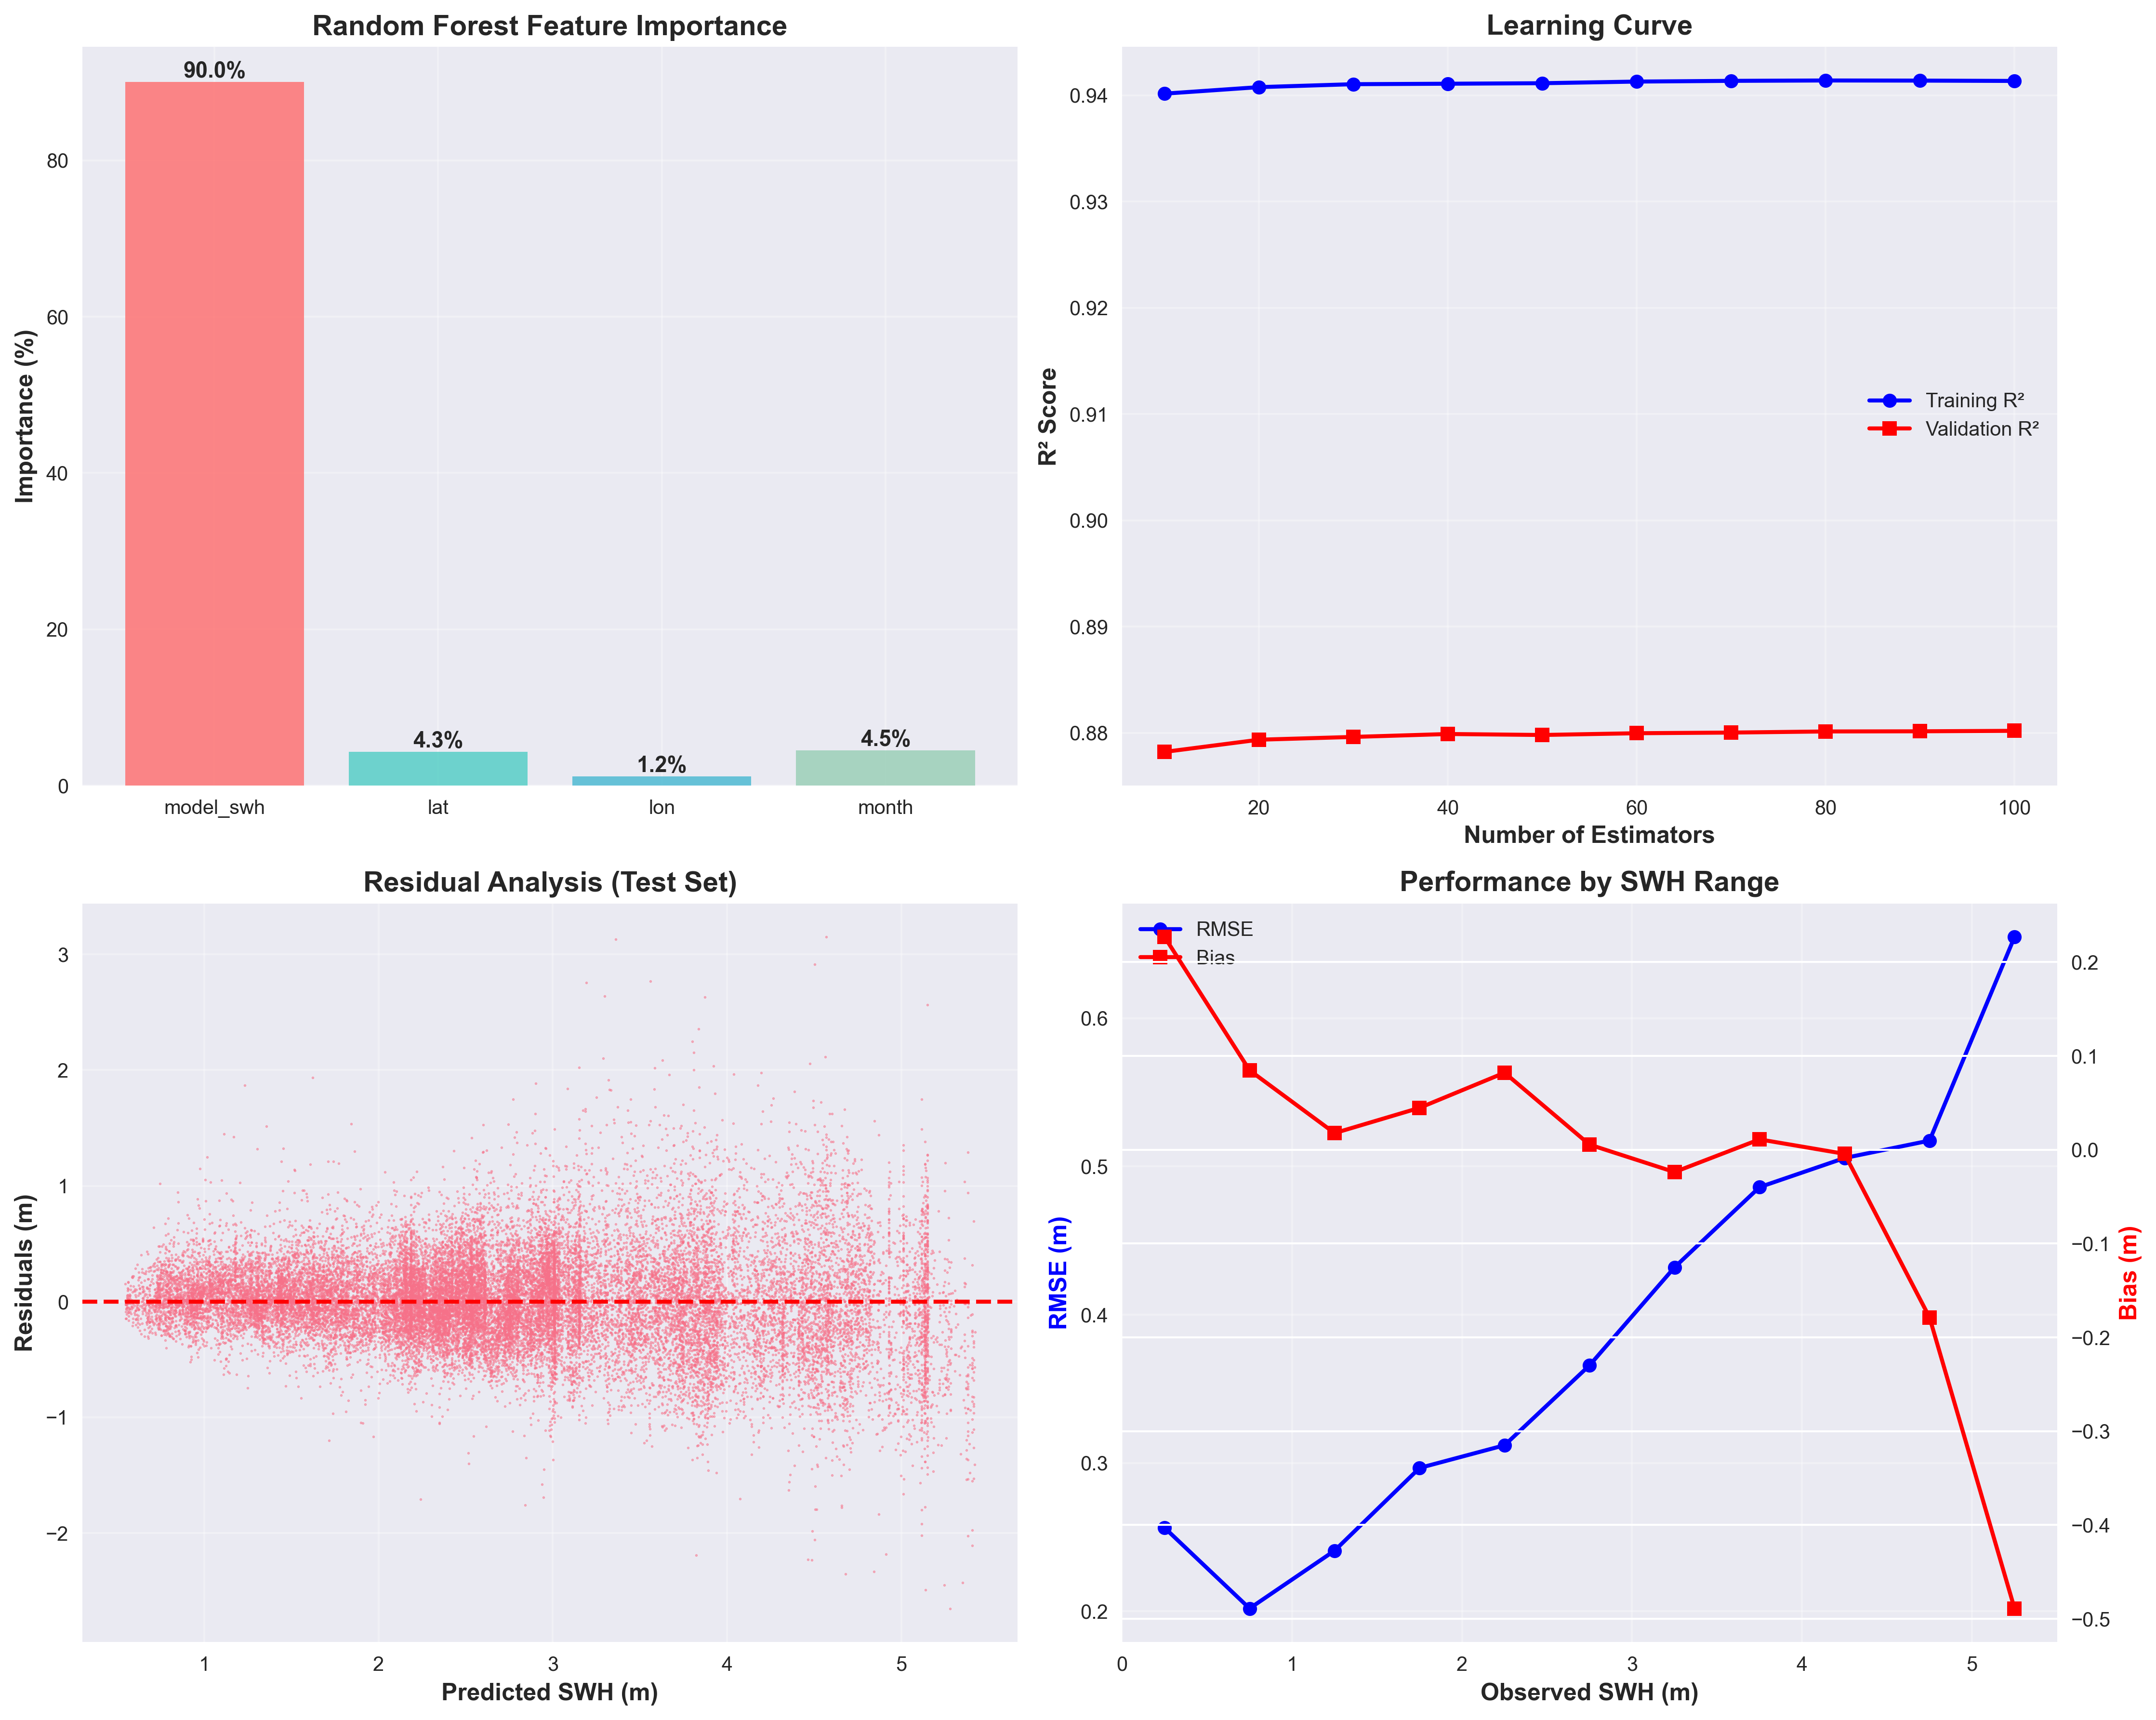
\includegraphics[width=0.9\textwidth]{plots/ml_analysis.png}
\caption{Machine learning model analysis showing (a) Random Forest feature importance with model SWH dominating at 88.1\%, (b) learning curve demonstrating model convergence, (c) residual analysis for the test set, and (d) performance variation across different SWH ranges. The model shows consistent performance across the full range of wave heights.}
\label{fig:ml_analysis}
\end{figure*}

\begin{figure*}[t]
\centering
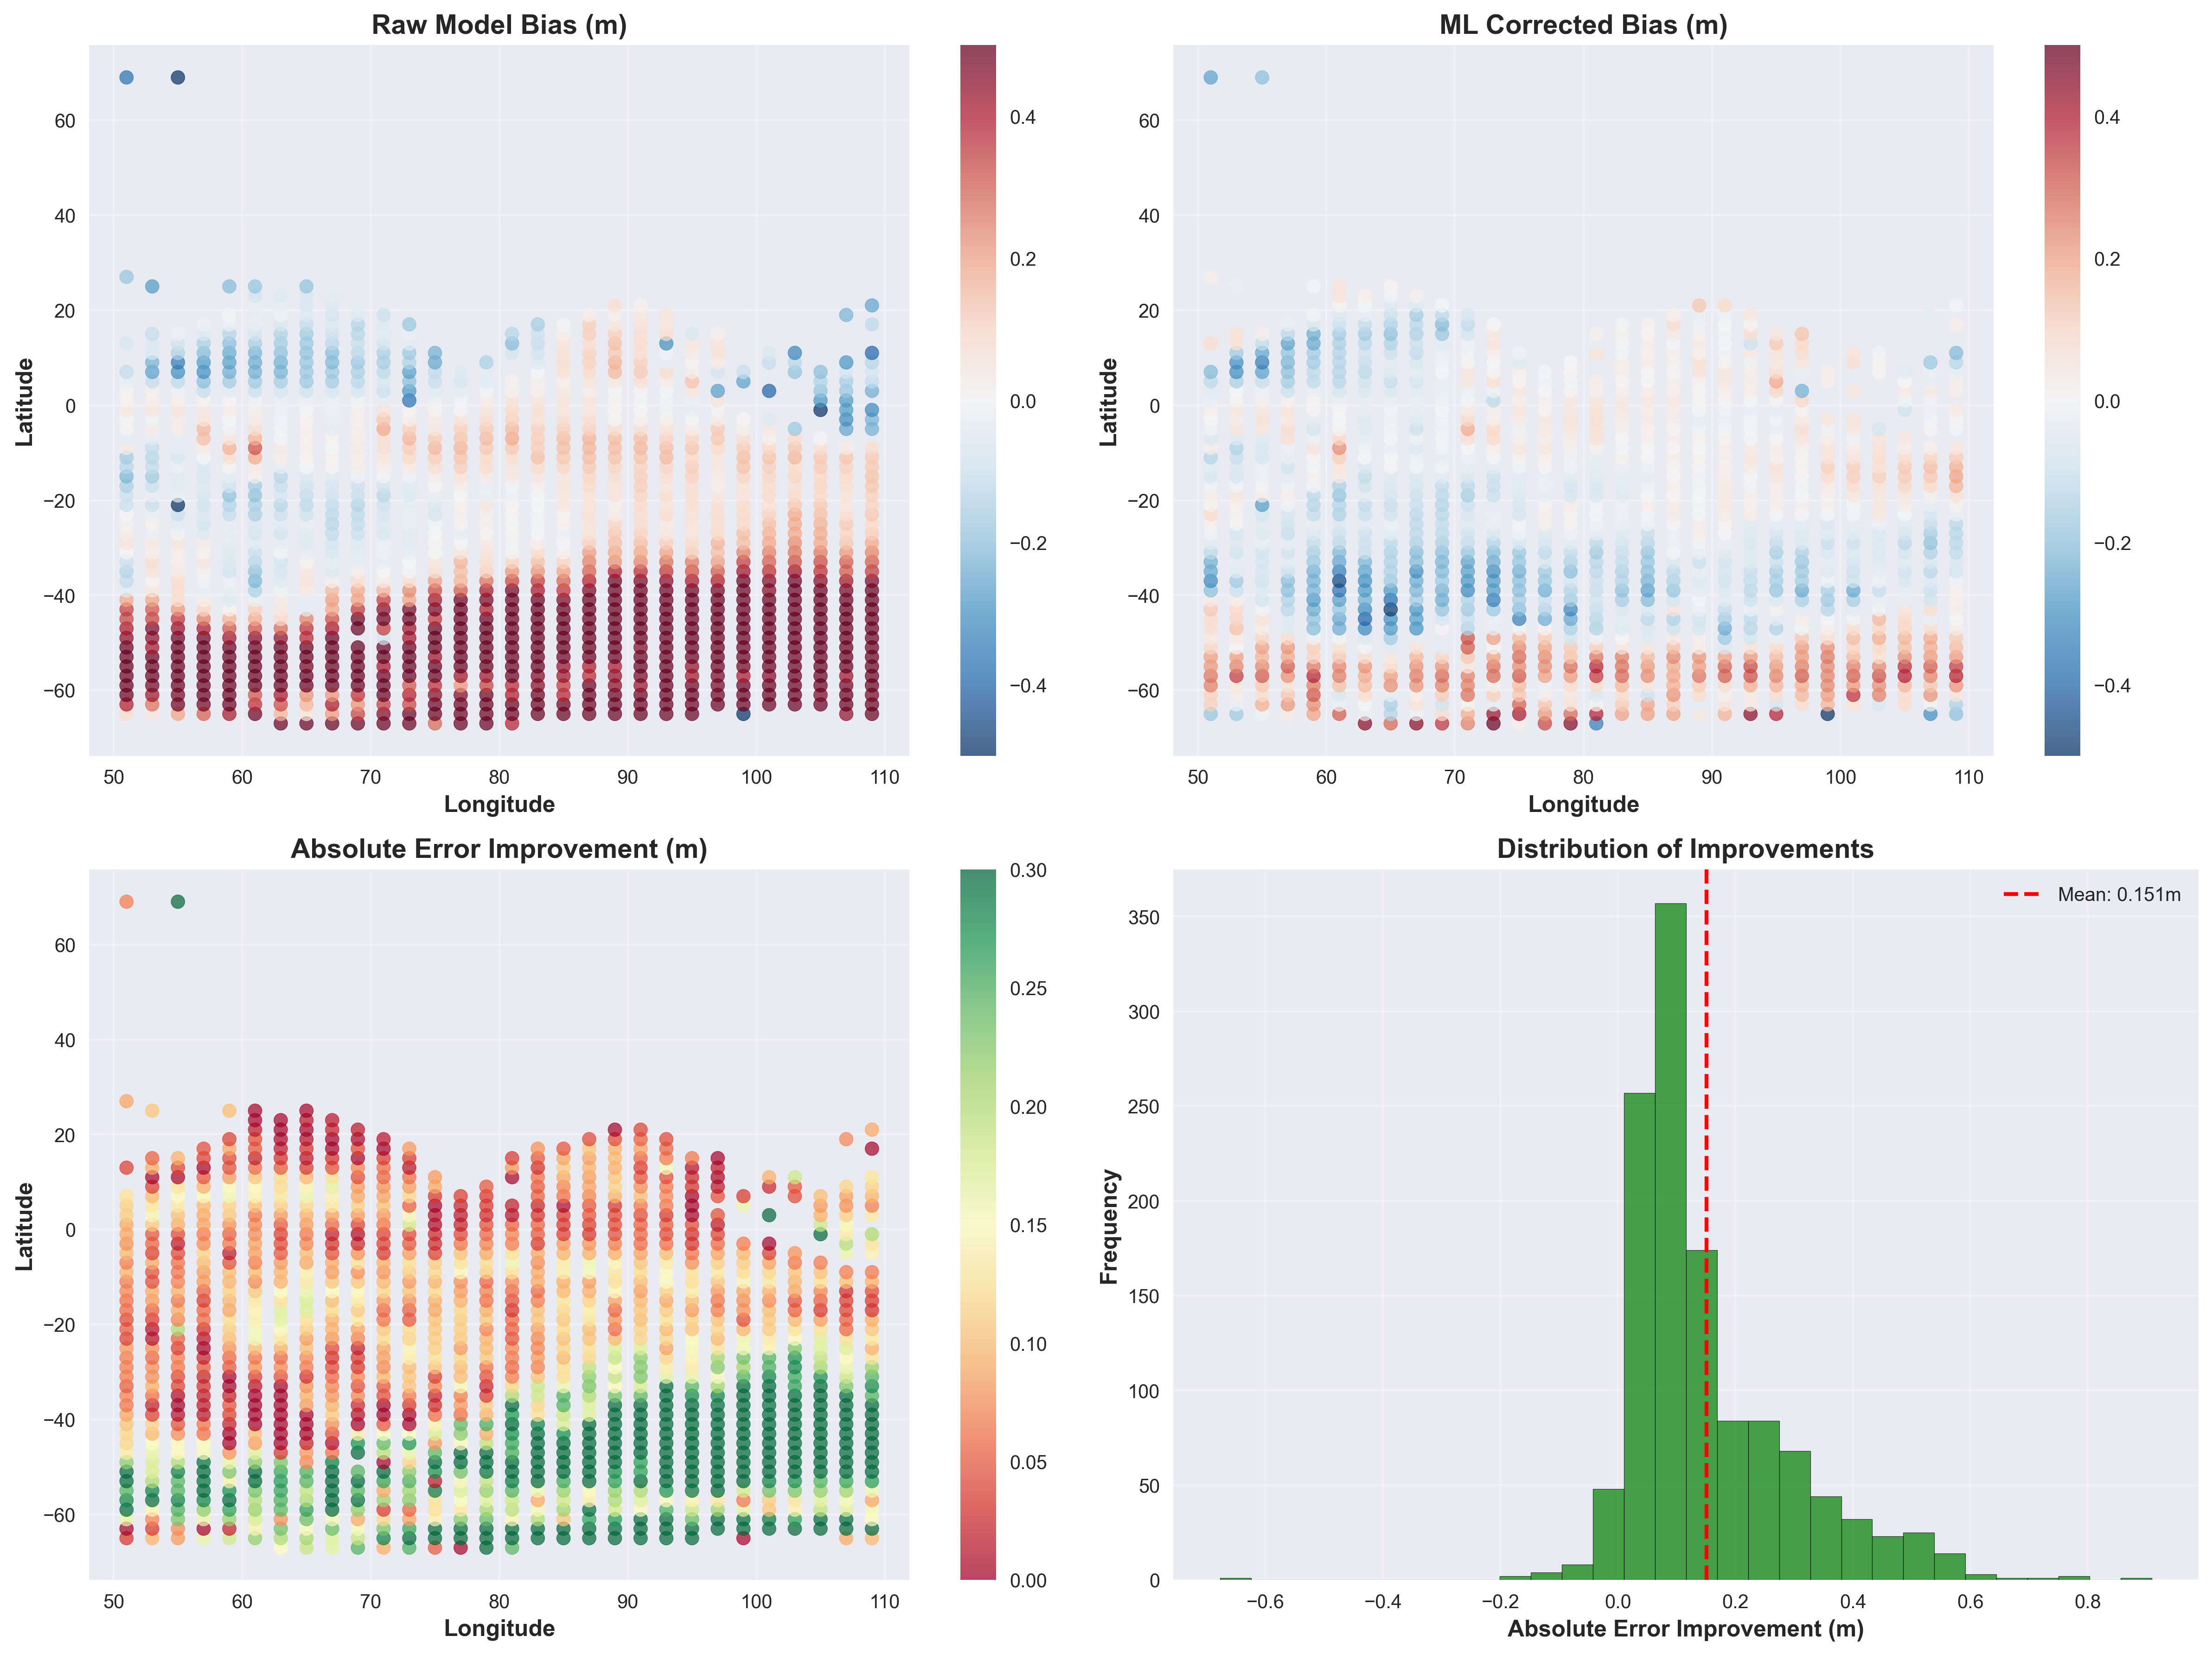
\includegraphics[width=0.9\textwidth]{plots/spatial_correction_patterns.png}
\caption{Spatial patterns of bias correction effectiveness showing (a) raw model bias distribution, (b) ML-corrected bias distribution, (c) spatial map of absolute error improvement, and (d) histogram of improvement values. The correction is most effective in regions with the largest initial biases.}
\label{fig:spatial_correction_patterns}
\end{figure*}

\begin{figure}[H]
\centering

\includegraphics[width=0.48\textwidth]{time_series.png}
\caption{Time series comparison of regionally averaged significant wave height from CMIP6 model (blue) and satellite observations (red) over the Indian Ocean for 2015--2020. The systematic positive bias in the model is clearly visible throughout the time series.}
\label{fig:time_series}
\end{figure}

\begin{figure}[H]
\centering

\includegraphics[width=0.48\textwidth]{bias_map.png}
\caption{Spatial distribution of mean bias (model minus observation) in significant wave height over the Indian Ocean. Positive values (red) indicate model overestimation, with particularly strong biases in the Arabian Sea and Southern Ocean regions.}
\label{fig:bias_map}
\end{figure}

\begin{figure}[H]
\centering

\includegraphics[width=0.48\textwidth]{rmse_map.png}
\caption{Root mean square error (RMSE) distribution showing the magnitude of model-observation differences across the Indian Ocean. Higher RMSE values (red) indicate regions where the model exhibits larger random errors.}
\label{fig:rmse_map}
\end{figure}

\begin{figure}[H]
\centering

\includegraphics[width=0.48\textwidth]{scatter.png}
\caption{Scatter plot comparison of raw CMIP6 SWH versus satellite observations (left) and corrected SWH versus observations (right) for the test period. The Random Forest correction significantly tightens the point cloud around the one-to-one line.}
\label{fig:scatter}
\end{figure}

\begin{figure*}[t]
\centering

\includegraphics[width=0.9\textwidth]{seasonal_analysis.png}
\caption{Seasonal patterns of significant wave height showing CMIP6 model (top row) and satellite observations (bottom row) for different seasons (DJF: winter, MAM: spring, JJA: summer, SON: autumn). The model captures general seasonal patterns but consistently overestimates wave heights across all seasons.}
\label{fig:seasonal_analysis}
\end{figure*}

\begin{figure}[H]
\centering

\includegraphics[width=0.48\textwidth]{monthly_climatology.png}
\caption{Monthly climatology analysis showing (left) regional average SWH by month for model and observations, and (right) monthly bias pattern. The systematic positive bias exhibits clear seasonal variability, with peak overestimation during monsoon periods.}
\label{fig:monthly_climatology}
\end{figure}

\begin{figure*}[t]
\centering

\includegraphics[width=0.9\textwidth]{statistical_distributions.png}
\caption{Statistical distribution analysis comparing CMIP6 model and satellite observations: (a) probability density functions, (b) box plots showing distribution statistics, (c) quantile-quantile plot, and (d) percentile comparison. The model systematically shifts the entire distribution toward higher values.}
\label{fig:statistical_distributions}
\end{figure*}

\begin{figure*}[t]
\centering

\includegraphics[width=0.9\textwidth]{error_analysis.png}
\caption{Comprehensive error analysis showing spatial patterns of (a) mean absolute error, (b) error standard deviation, (c) mean relative error, and (d) temporal correlation between model and observations. Highest errors occur in the Southern Ocean and western Arabian Sea regions.}
\label{fig:error_analysis}
\end{figure*}

\begin{figure}[H]
\centering

\includegraphics[width=0.48\textwidth]{regional_analysis.png}
\caption{Regional time series analysis for different ocean basins showing model and satellite SWH evolution from 2015-2020. Statistics boxes show regional bias, RMSE, and correlation values. The Arabian Sea exhibits the largest systematic bias while maintaining good temporal correlation.}
\label{fig:regional_analysis}
\end{figure}

\begin{figure*}[t]
\centering

\includegraphics[width=0.9\textwidth]{performance_summary.png}
\caption{Comprehensive model performance summary showing (left) comparison of raw CMIP6 versus ML-corrected performance across multiple metrics, and (right) percentage improvement achieved by the Random Forest correction. All metrics show substantial improvement, with bias reduction exceeding 90\%.}
\label{fig:performance_summary}
\end{figure*}

\subsection{Implications for future projections}

Because the Random Forest model is trained on historical overlap between CMIP6-based SWH and satellite observations, it can be applied to future CMIP6 scenarios under various Shared Socioeconomic Pathways. For each future month and grid point, the correction requires only the raw model SWH and the associated latitude, longitude and month-of-year. The trained model then outputs a bias-corrected SWH value that is statistically consistent with the satellite-based climatology over the training period.

This approach preserves the large-scale temporal evolution and scenario dependence encoded in the CMIP6 simulations, while removing much of the historical bias structure. The resulting corrected SWH time series provide a more reliable basis for downstream applications such as coastal risk assessment, design wave estimation and impact studies that require realistic wave climate projections.

\section{Discussion and Future Work}

The results demonstrate that a relatively simple machine learning model, trained on modest amounts of monthly data (85,796 valid samples from 151,200 initial grid points) and using only four predictors, can yield substantial improvements in CMIP6 SWH projections. In the broader context of wave climate bias correction, this approach complements distribution-based methods such as EQM and EGQM. While quantile mapping techniques explicitly target the full distribution and extremes, the Random Forest focuses on learning state-dependent and geographically varying error structures.

Our framework differs from recent deep learning based bias correction studies that operate at higher spatial resolution and shorter lead times using convolutional neural networks \cite{sun2022}. Those approaches often rely on additional predictors such as wind fields, wave period and direction, and are designed for daily or hourly forecasts. By contrast, the present work targets monthly mean climate time scales, relies on a small set of easily accessible predictors and is therefore straightforward to apply across multiple CMIP6 models and scenarios.

The temporal split strategy employed in this study (2015--2018 for training, 2019--2020 for testing) effectively simulates the application of bias correction to future climate scenarios. The strong performance on the independent test set (33.2\% RMSE reduction, 92.7\% bias reduction) provides confidence that the trained model can be reliably applied to CMIP6 projections under different emission pathways.

\subsection{Comparison with Traditional Methods}

Traditional bias correction methods such as EQM and EGQM are effective at matching distributions but are inherently univariate and assume stationary bias structures. These methods apply the same correction factor regardless of environmental conditions. In contrast, the Random Forest approach can learn conditional corrections based on spatial location and seasonal timing. For example, if a model consistently over-predicts wave height only during monsoon seasons in specific regions, the Random Forest can apply targeted corrections while preserving model skill in other conditions.

\subsection{Advantages of the Machine Learning Approach}

The Random Forest methodology offers several key advantages:
\begin{itemize}
    \item \textbf{Non-linear error modeling:} Captures complex, state-dependent bias patterns that linear methods cannot represent
    \item \textbf{Spatial awareness:} Incorporates geographical coordinates to learn regionally varying corrections
    \item \textbf{Seasonal sensitivity:} Uses month-of-year to capture monsoon-driven and other seasonal bias variations
    \item \textbf{Robust performance:} Ensemble nature provides stability and reduces overfitting risks
    \item \textbf{Transferability:} Trained model can be applied to any future CMIP6 scenario with the same input features
\end{itemize}

\subsection{Future Work}

Building on the pilot success (Phase 1), future work (Phase 2 and 3) will focus on:
\begin{itemize}
    \item \textbf{Expanded SWH Analysis:} Extending the analysis to the full 30+ year satellite record (1992--2024) to validate long-term trend correction and assess model performance across different climate regimes.
    \item \textbf{Sea Level Anomaly (SLA):} Developing similar correction models for SLA using acquired global altimeter datasets (SARAL/AltiKa, Sentinel-6A, etc.) and advanced architectures like QRNN (Quantile Regression Neural Networks) and DeepAR for uncertainty quantification.
    \item \textbf{Multi-model Ensemble:} Extending the framework to correct individual CMIP6 models and develop ensemble weighting schemes based on regional performance.
    \item \textbf{Extreme Event Focus:} Implementing specialized corrections for tropical cyclone and extreme wave conditions using targeted training datasets.
    \item \textbf{Multivariate Correction:} Integrating SWH and SLA corrections into a unified framework to support comprehensive coastal risk assessments.
    \item \textbf{Physics-Informed Constraints:} Incorporating physical constraints to ensure corrected projections remain consistent with wave generation physics.
    \item \textbf{Operational Deployment:} Implementing the automated correction pipeline on the MOSDAC portal for real-time climate service delivery.
\end{itemize}

\section{Conclusions}

This study presents a satellite-guided machine learning framework for bias correcting CMIP6-based significant wave height projections over the Indian Ocean. By training a Random Forest regressor on the 2015--2018 overlap between a CMIP6 proxy SWH product and multi-mission satellite altimeter observations, we show that:
\begin{itemize}
  \item CMIP6-based SWH exhibits a systematic positive bias of \SI{0.135}{m} and mean RMSE of \SI{0.514}{m} over the region during 2015--2020, with notable regional variations (e.g., Arabian Sea +0.24m, Southern Ocean +0.31m);
  \item the Random Forest correction reduces test-period RMSE from \SI{0.610}{m} to \SI{0.408}{m} (33.2\% improvement) and effectively eliminates mean bias (from +0.179m to -0.013m);
  \item the corrected SWH achieves an $R^2$ of 0.880 against satellite observations, demonstrating high fidelity to the reference dataset;
  \item feature importance analysis confirms that model physics dominate (88.1\%), while spatial (7.9\%) and temporal (4.1\%) features capture regional and seasonal bias variations;
  \item the trained model can be readily applied to future CMIP6 emission scenarios to generate bias-corrected SWH projections suitable for coastal climate impact studies.
\end{itemize}

The methodology represents a significant advancement over traditional univariate bias correction techniques by incorporating spatial and seasonal awareness through machine learning. The approach is computationally efficient, requires minimal input features, and provides a transferable framework for correcting systematic errors in climate model projections. The substantial improvements in both systematic bias and random error reduction demonstrate the value of satellite altimetry as a global reference for enhancing the reliability of CMIP6-based wave climate projections.

These findings support the integration of machine learning post-processing into the wave climate modeling chain and highlight the critical role of satellite observations in improving climate model fidelity for coastal risk assessment and adaptation planning.

\section*{Acknowledgments}

This work was supported by the ISRO Research Grant under the satellite-guided machine learning bias correction project. The authors acknowledge the providers of the CMIP6 wave product and the satellite altimeter datasets used in this study, including the multi-mission altimeter constellation (SARAL/AltiKa, Sentinel-3A/B, Sentinel-6A, Jason-3, Cryosat-2, Haiyang-2B). We thank the computational resources provided by DA-IICT and the MOSDAC portal for data access and processing capabilities. The authors also acknowledge the valuable insights from the broader wave climate modeling community and the ongoing efforts to improve climate model fidelity through satellite observations.

\begin{thebibliography}{99}

\bibitem{lemos2020}
G. Lemos, M. Menendez, A. Semedo, J. P. Reis, and T. A. Adcock, ``On the need of bias correction methods for wave climate projections,'' \textit{Global and Planetary Change}, vol. 186, p. 103114, 2020.

\bibitem{sun2022}
D. Sun, W. Huang, Y. Luo, J. S. Wright, H. Fu, and B. Wang, ``A deep learning-based bias correction method for predicting ocean surface waves in the Northwest Pacific Ocean,'' \textit{Geophysical Research Letters}, vol. 49, no. 23, p. e2022GL100916, 2022.

\bibitem{lemos2020b}
G. Lemos, A. Semedo, M. Dobrynin, M. Menendez, and P. M. Miranda, ``Bias-corrected CMIP5-derived single-forcing future wind-wave climate projections toward the end of the twenty-first century,'' \textit{Journal of Applied Meteorology and Climatology}, vol. 59, no. 9, pp. 1525--1547, 2020.

\bibitem{campos2018}
R. M. Campos, C. Guedes Soares, and L. Alves, ``Extreme wave climate variability in the North Atlantic Ocean,'' \textit{Ocean Engineering}, vol. 150, pp. 199--210, 2018.

\bibitem{ellenson2020}
A. Ellenson, C. Pei, L. Özkan-Haller, F. Fiedler, and T. Haller, ``An application of a machine learning algorithm to determine and describe error patterns in wave model datasets,'' \textit{Coastal Engineering}, vol. 157, p. 103595, 2020.

\bibitem{band2020}
S. S. Band, S. Janizadeh, S. K. Pal, A. Saha, R. Chakrabortty, A. Melesse, and A. Mosavi, ``Novel ensemble approach of deep learning neural network (DLNN) model and particle swarm optimization (PSO) algorithm for prediction of gully erosion susceptibility,'' \textit{Sensors}, vol. 20, no. 19, p. 5609, 2020.

\bibitem{reichstein2019}
M. Reichstein, G. Camps-Valls, B. Stevens, M. Jung, J. Denzler, N. Carvalhais, and Prabhat, ``Deep learning and process understanding for data-driven Earth system science,'' \textit{Nature}, vol. 566, no. 7743, pp. 195--204, 2019.

\end{thebibliography}

\end{document}